\chapter{Algorithm (change name)}


%%%%%%%%%%%%%%%%%%%%%%%%%%%%%%%%%%%%%%%%%%%%%
\section{Motivation}
\whendraft{
\begin{enumerate}
    \item Why create the algorithm ?
    \begin{itemize}
        \item We wanted a way to explore structures.
    \end{itemize}
    
\end{enumerate}
}

%%%%%%%%%%%%%%%%%%%%%%%%%%%%%%%%%%%%%%%%%%%%%
\section{Description [/preliminaries?]}
\whendraft{
\textbf{Include in algorithm description:}
\begin{enumerate}
    \item Make up of $\mathcal{E}$.
    \item We store actions as their unique sequences of minimum actions.
    \item All we need from $\mathscr{W}$ is the set $W$ of world states and the map $\hat{*}: \hat{A} \times W \to W$.
    We treat $\hat{*}$ as a part of $\mathscr{W}$.
    \item How we use the $\operatorname{Combine}$ operator to evaluate $\circ$.
    \item What each of elements of $\mathcal{E}$ are at the termination of the algorithm.
    \item $\operatorname{Seq} : \hat{A}^* \to (\hat{A})^n, \quad \operatorname{Seq}(a) = (\hat{a}_{n}, \hat{a}_{n-1}, \dots, \hat{a}_{1})$
    \item Explain how assignment to $\mathcal{E}$ works - assignment occurs for each of the constituents of $\mathcal{E}$.
    \item Mention that the only bit of information needed from $\mathscr{W}$ is the mapping: $\hat{*}: \hat{A} \times W \to W$ that takes a minimum action and applies it to a world state.
\end{enumerate}

\begin{enumerate}
    \item Change name of `states Cayley table' and `actions Cayley table` ?
    \begin{itemize}
        \item Cayley table is already a thing.
    \end{itemize}
\end{enumerate}
}


%%%%%%%%%%%%%%%%%%%%%%%%%%%%%%%%%%%%%%%%%%%%%
\subsection{The initial}


The definition of $\sim$ is ...





%%%%%%%%%%%%%%%%%%%%%%%%%%%%%%%%%%%%%%%%%%%%%
\section{Mathematical preliminaries}
\whendraft{
\begin{enumerate}
    \item Definition of Cayley table. - put this in motivation section ?
\end{enumerate}
}


\paragraph{What is an actions Cayley table?}




%%%%%%%%%%%%%%%%%%%%%%%%%%%%%%%%%%%%%%%%%%%%%
\subsection{Design decisions}

\paragraph{Problem:}
[?] Assessing equality between two actions.
\\\textit{Solution:}


\paragraph{Problem:}
Calculating the result of the $\circ$ operator.
\\\textit{Solution:}



%%%%%%%%%%%%%%%%%%%%%%%%%%%%%%%%%%%%%%%%%%%%%
%%%%%%%%%%%%%%%%%%%%%%%%%%%%%%%%%%%%%%%%%%%%%
%%%%%%%%%%%%%%%%%%%%%%%%%%%%%%%%%%%%%%%%%%%%%

\paragraph{Problem:}
How do we know if the algebra produced is complete?
\\\textit{Solution:}
\begin{itemize}
    \item 
\end{itemize}


\paragraph{Problem:}
Dealing with undefined actions.
\\\textit{Solution:}
\begin{itemize}
    \item Describe how we implemented the undefined state.
\end{itemize}




%%%%%%%%%%%%%%%%%%%%%%%%%%%%%%%%%%%%%%%%%%%%%
\section{Pseudocode}
\whendraft{
\noindent\rule{\textwidth}{1mm}
\textbf{To do:}
\begin{enumerate}
    \item [visual] Span algorithms across entire page.
\end{enumerate}
\noindent\rule{\textwidth}{1mm}
}


\begin{table}[H]
\begin{tabularx}{\textwidth}{lX}
\toprule
\textbf{Symbol} & \textbf{Description} \\
\midrule
$\hat{A}$ & The set of minimum actions of the agent. Elements of $\hat{A}$ are given a $\hat{\ }$. \\
$\mathscr{W} = (W, \; \hat{\ast})$ & The world characterised by a set $W$ of world states and a minimum action effect map $\hat{\ast}$. \\
$W$ & The set of world states. \\
$\hat{\ast}$ & The minimum effect map $\hat{A} \times W \to W$ that sends a minimum action-world state pair to the resultant world state after the agent performs that minimum action in the world state. \\
$L$ & The set of equivalence class labels. \\
$E$ & The set of processed elements. These elements have been assigned to a equivalence class labelled by $L$. \\
$\pi$ & A map $E \to L$ that sends each processed element $a \in E$ to its equivalence class labelling element $l \in L$. \\
$\mathcal{E} = (L, \; E, \; \pi)$ & The equivalence classes. \\
$\mathcal{T}$ & A set of functions $f_{a}: W \to W$, where $a \in L$. \\
$\rho$ & A map $L \to \mathcal{T}$ such that $\rho(l) = f_{l}$. \\
$\hat{A}/\sim$ & The set of minimum actions that are distinct under $\sim$. \\
$n$ & Counter that represents the length of the current candidate action sequences. \\
$N_{L}$ & The number of new equivalence class labelling elements found in the current iteration. \\
$A_{C}$ & The set of elements that are candidates for new equivalence class labelling elements in $L$. Candidate elements are denoted by $a_{C}$. \\
$\mathcal{L}_{n}(L)$ & A filtering map $L \to \{ l \in L \mid |l| = n \}$ that filters the elements of a set $L$ of actions to leave the actions that are of length $n$. \\
$\operatorname{Combine}$ & The combine operator that combines two sequences of minimum actions as $\operatorname{Combine}((a_{p}, \; \dots \;, \; a_{1}), \; (b_{k}, \; \dots \; , \; b_{1})) = (a_{p}, \; \dots \; , \; a_{1}, \; b_{k}, \; \dots \; , \; b_{1})$. \\
$T_{A}$ & The Cayley table. \\
\bottomrule
\end{tabularx}
\caption{Key for pseudocode.}
\label{tab:pseudocode_key}
\end{table}


\begin{table}[H]
    \centering
    \begin{tabular}{c|c}
        a & b \\
        c & d
    \end{tabular}
    \caption{Caption}
    \label{tab:my_label}
\end{table}


\begin{figure}[H]
    \centering
    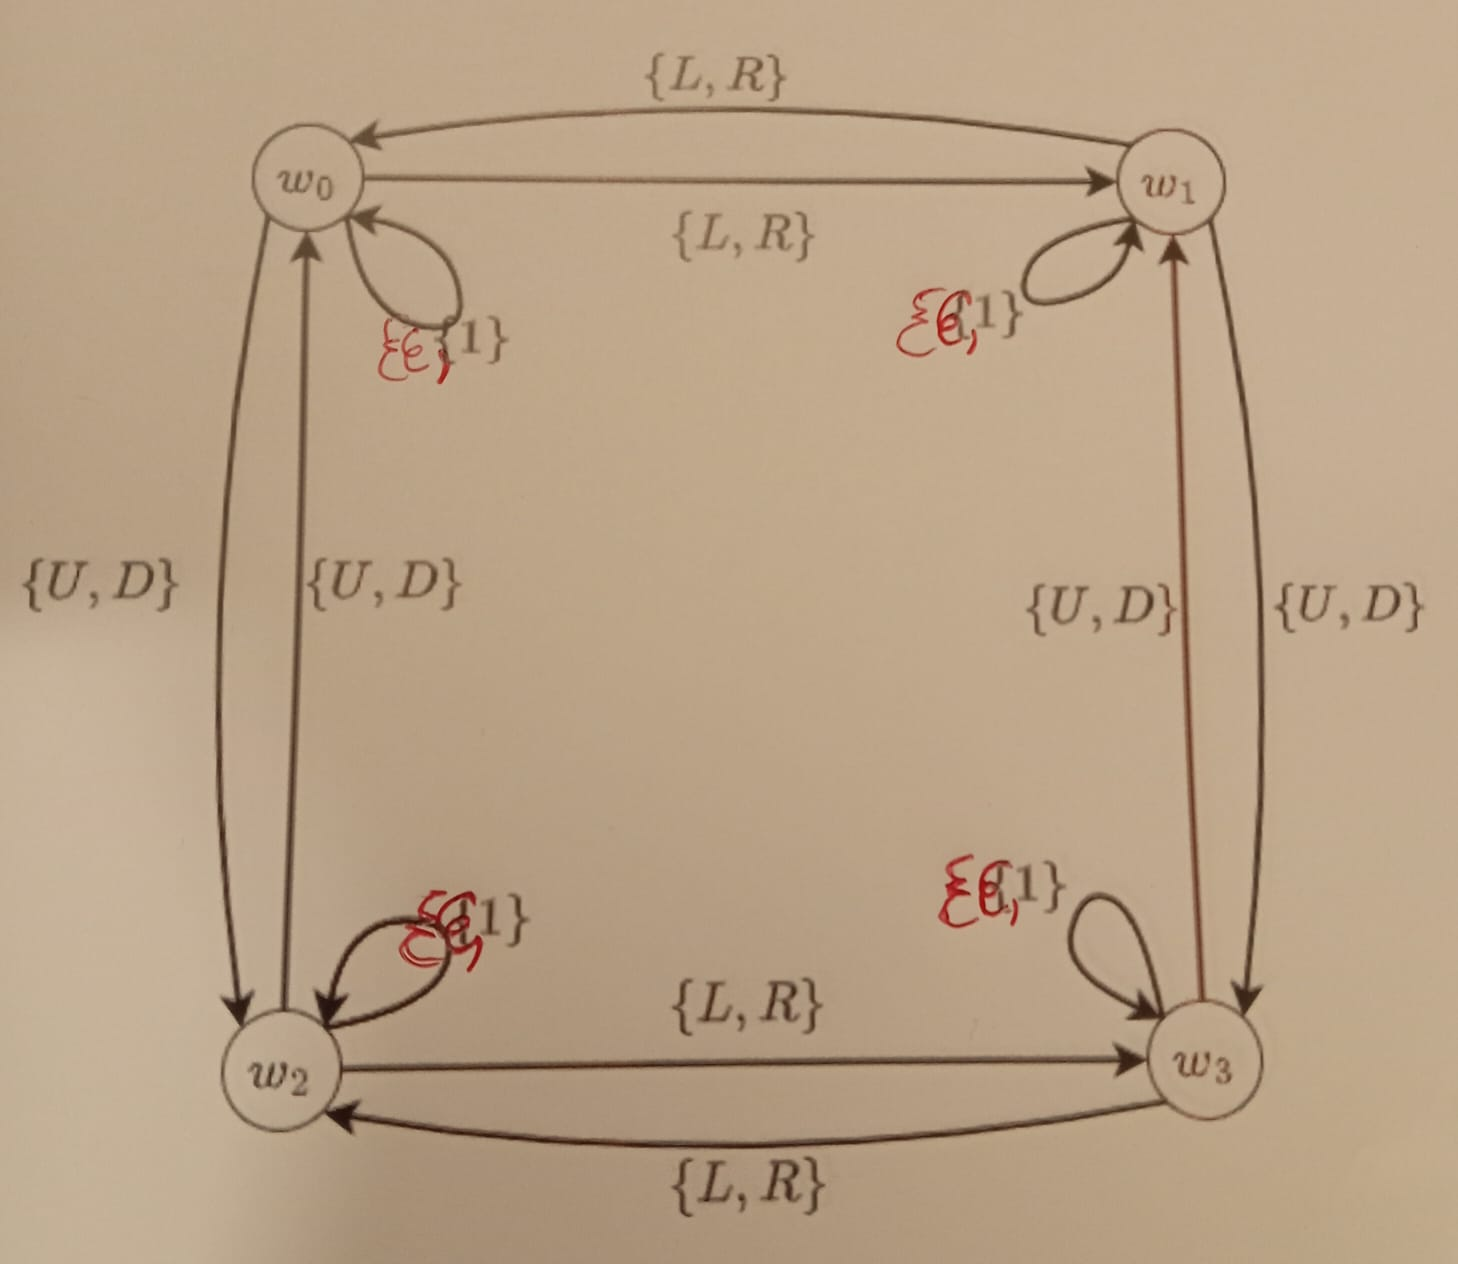
\includegraphics[width=0.5\linewidth]{2MathematicalFramework/InitialFramework/Images/2x2_cyclical_equivalence_min_actions.jpeg}
    \caption{Caption}
    \label{fig:enter-label}
\end{figure}


%%%%%%%%%%%%%%%%%%%%%%%%%%%%%%%%%%%%%%%%%%%%%
\subsection{Generate equivalence classes}

\begin{algorithm}[H]
\caption{
Generate the equivalence classes $\mathcal{E} = (L, \; E, \; \pi: E \to L)$ for $\sim$ and the set of action functions $\mathcal{T} = \{f_{l}: W \to W\}$ for a world $\mathscr{W} = (W, \; \hat{\ast})$ that is characterised by a set $W$ of world states and a minimum action effect map $\hat{\ast}$.
}
\hrulefill
\begin{algorithmic}[1]
\Procedure{GenerateEquivClasses}{$\hat{A}$, \; $\mathscr{W}$}
    \Statex \Comment{Initialise equivalence classes object $\mathcal{E}$.}
    \State $L \gets \emptyset$
    \State $E \gets \emptyset$
    \State $\pi \gets (\emptyset \to \emptyset)$
    \State $\mathcal{E} \gets (L, \; E, \; \pi)$.

    \Statex \Comment{Initialise $\mathcal{T}$ and $\rho$}
    \State $\mathcal{T} \gets \emptyset$
    \State $\rho: \gets (\emptyset \to \emptyset)$

    \Statex \Comment{Find distinct minimum actions.}
    \For{\textbf{each} $\hat{a} \in \hat{A}$}
        \State $(\mathcal{E}, \; \mathcal{T}, \; \rho) \gets$ \Call{ProcessCandidate}{$\hat{a}$, \; $\mathcal{T}$, \; $\rho$, \; $\mathcal{E}$, \; $\mathscr{W}$}
    \EndFor
    \State $\hat{A}/\sim \; \gets L$

    \Statex \Comment{Iteratively create candidate actions sequences for equivalence class labelling elements then check if they are successful candidates.}
    \State $n \gets 0$
    \State $N_{L} \gets 0$
    \Statex \Comment{If no new labelling actions found in a set of candidate elements, then halt the algorithm.}
    \While{$N_{L} \neq |L|$}
        \State $n \gets n + 1$
        \State $N_{L} \gets |L|$
        \State $A_{C} \gets \Call{GenerateCandidates}{\mathcal{L}_{n}(L), \;  \hat{A}/\sim}$

        \For{\textbf{each} $a_{C} \in A_{C}$}
            \State $(\mathcal{E}, \; \mathcal{T}, \; \rho) \gets$ \Call{ProcessCandidate}{$a_{C}$, \; $\mathcal{T}$, \; $\rho$, \; $\mathcal{E}$, \; $\mathscr{W}$}
        \EndFor
    \EndWhile
    \State \Return $\mathcal{E}, \; \mathcal{T}$
\EndProcedure
\end{algorithmic}
\end{algorithm}


\begin{algorithm}[H]
\caption{
Generate new action sequences that are candidates for equivalence class labelling elements.
}
\hrulefill
\begin{algorithmic}[1]
\Procedure{GenerateCandidates}{$L$, \;  $\hat{A}/\sim$}
    \State $A_{C} \gets \emptyset$
    \ForAll{$(l, \; \hat{a}) \in L \times \hat{A}/\sim$}
            \State $a' = \operatorname{Combine}(\hat{a}, \; l)$
            \State $A_{C} \gets A_{C} \cup \{a'\}$
    \EndFor
    \State \Return $A_{C}$
\EndProcedure
\end{algorithmic}
\end{algorithm}


\begin{algorithm}[H]
\caption{
Process a candidate $a_{C}$ for being an equivalence class labelling element.
If $a_{C}$ is a successful candidate, then create a new equivalence classes labelled by $a_{C}$.
If $a_{C}$ is found to be in another equivalence class then add it to that equivalence class.
}
\hrulefill
\begin{algorithmic}[1]
\Procedure{ProcessCandidate}{$a_{C}$, \; $\mathcal{T}$, \; $\rho$, \; $\mathcal{E}$, \; $\mathscr{W}$}
    \State $f_{a_{C}} = \Call{ComputeActionFunction}{a_{C}, \; \mathscr{W}}$

    \If{$f_{a_{C}} \in \mathcal{T}$}
        \Statex \Comment{Add $a_{C}$ to equivalence class in $\mathcal{E}$ with class label that has the same action function $f_{a_{C}}$.}
        \State $\mathcal{E} \gets (\; L, \; E \cup \{a_{C}\}, \; \pi \cup \pi' \;)$, where $\pi': \{a_{C}\} \to L$ such that $\pi'(a_{C}) = \rho^{-1}(f_{a_{C}})$.
    \Else
        \Statex \Comment{Create new equivalence class in $\mathcal{E}$ labelled by $a_{C}$.}
        \State $\mathcal{E}' \gets (\; L \cup \{a_{C}\}, \; E \cup \{a_{C}\}, \; \pi \cup \pi' \;)$, where $\pi': \{a_{C}\} \to \{a_{C}\}$ such that $\pi'(a_{C}) = a_{C}$.

        \Statex \Comment{Add $f_{a_{C}}$ to $\mathcal{T}$.}
        \State $\mathcal{T}' \gets \mathcal{T} \cup \{f_{a_{C}}\}$

        \Statex \Comment{Update $\rho$ to send $a_{C}$ to $f_{a_{C}}$.}
        \State $\rho' \gets \rho \cup \rho''$ where $\rho'': \{a_{C}\} \to \{f_{a_{C}}\}$ such that $\rho''(a_{C}) = f_{a_{C}}$
    \EndIf
    \State \Return $(\mathcal{E}', \; \mathcal{T}', \; \rho')$
\EndProcedure
\end{algorithmic}
\end{algorithm}



\begin{algorithm}[H]
\caption{Compute the action function $f_{a}: W \to W$ that sends $w \mapsto a \ast w$.}
\hrulefill
\begin{algorithmic}[1]
\Procedure{ComputeActionFunction}{$a$, \; $\mathscr{W}$}
    \State $f_{a} \gets (\emptyset \to \emptyset)$
    \ForAll{$w \in W$}
        \State $w_{a} \gets$ \Call{GenerateActionOutcome}{$a$, \; $w$, \; $\hat{\ast}$}
        \State $f_{a} \gets f_{a} \cup f_{a}'$ where $f_{a}': \{w\} \to \{w_{a}\}$ such that $f_{a}'(w) = w_{a}$
    \EndFor
    \State \Return $f_{a}$
\EndProcedure
\end{algorithmic}
\end{algorithm}


\begin{algorithm}[H]
\caption{
Generate the outcome state of a world $\mathscr{W}$ when an action sequence $a$ is applied to the world in an initial state $w$.
}
\label{alg:GenerateActionOutcome}
\hrulefill
\begin{algorithmic}[1]
\Procedure{GenerateActionOutcome}{$a$, \; $w$, \; $\hat{\ast}$}
    \State $w_{a} \gets w$
    \For{$i \gets 1, \; \dots \;, \; n$}
        \State $w_{a} \gets \hat{a}_{i} \; \hat{\ast} \; w_{a}$ where $\operatorname{Seq}(a) = (\hat{a}_n, \; \hat{a}_{n-1}, \; \dots \;, \; \hat{a}_1)$
    \EndFor
    \State \Return $w_{a}$
\EndProcedure
\end{algorithmic}
\end{algorithm}


%%%%%%%%%%%%%%%%%%%%%%%%%%%%%%%%%%%%%%%%%%%%%
\subsection{Generate Cayley table}

\begin{algorithm}[H]
\caption{
Generate the Cayley table $T_{A}$
}
\hrulefill
\begin{algorithmic}[1]
\Procedure{GenerateCayley}{$\mathcal{E}$}
    \State $T_{A} \gets$ Empty $|L| \times |L|$ table with rows and columns labelled by the elements of $L$.
    \Statex \Comment{Fill actions Cayley table.}
    \For{\textbf{each} $l_{row} \in L$}
        \For{\textbf{each} $l_{col} \in L$}
            \Statex \Comment{Get action function for the combined element.}
            \State $f_{(l_{col} \; \circ \; l_{row})} \gets$ \Call{ComputeCombinedActionFunction}{$l_{row}$, \; $l_{col}$, \; $\mathcal{T}$, \; $\rho$}
            \State $l \gets \rho^{-1}(f_{(l_{col} \; \circ \; l_{row})})$
            \State $T_{A}[l_{row}][l_{col}] \gets l$

            \whendraft{
            \Statex \Comment{TODO: Add $a$ to the equivalence class as $\operatorname{Combine}(l_{col}, l_{row})$?}
            \Statex \Comment{TODO: Include equivalence class check before generating the combined action function ?}
            }
            
        \EndFor
    \EndFor
    
    \State \Return $T_{A}$
\EndProcedure
\end{algorithmic}
\end{algorithm}


\begin{algorithm}[H]
\caption{
Compute the action function for the combination $l_{L} \circ l_{R}$ of two actions by combining their action functions.
}
\hrulefill
\begin{algorithmic}[1]
\Procedure{ComputeCombinedActionFunction}{$l_{R}$, \; $l_{L}$, \; $\mathcal{T}$, \; $\rho$}
    \Statex \Comment{Get action functions for $l_{R}$ and $l_{L}$.}
    \State $f_{R} \gets \rho(l_{R})$
    \State $f_{L} \gets \rho(l_{L})$
    
    \State $f_{a} \gets (\emptyset \to \emptyset)$
    \Statex \Comment{Compute the combined action function $f_{a}$}
    \State $f_{a} \gets (\emptyset \to \emptyset)$
    \ForAll{$w_{R, \; I} \in \operatorname{Dom}(f_{R})$}
        \State $w_{R, \; F} \gets f_{R}(w_{R, \; I})$
        \ForAll{$w_{L, \; I} \in \operatorname{f_{L}}$}
            \If{$w_{L, \; I} = w_{R, \; F}$}
                \State $w_{L, \; F} \gets f_{L}(w_{L, \; I})$
                \State $f_{a} \gets f_{a} \cup f_{a}'$ where $f_{a}': \{w_{R, \; I}\} \to \{w_{L, \; F}\}$ such that $f_{a}'(w_{R, \; I}) = w_{L, \; F}$
            \EndIf
        \EndFor
    \EndFor
    \State \Return $f_{a}$
\EndProcedure
\end{algorithmic}
\end{algorithm}

%%%%%%%%%%%%%%%%%%%%%%%%%%%%%%%%%%%%%%%%%%%%%
\whendraft{
\section{Example [\textbf{To do}]}
}

%%%%%%%%%%%%%%%%%%%%%%%%%%%%%%%%%%%%%%%%%%%%%
\section{Mathematical justification}
\whendraft{
\noindent\rule{\textwidth}{1mm}
\textbf{To do:}
\begin{enumerate}
    \item Proof that algorithm halts when it has all necessary elements and not before.
\end{enumerate}
\noindent\rule{\textwidth}{1mm}
}



%%%%%%%%%%%%%%%%%%%%%%%%%%%%%%%%%%%%%%%%%%%%%
\section{Minimum actions affect the algebra}
\whendraft{
\begin{enumerate}
    \item Have a world $\mathscr{W}$ with loads of transformations, then have different agent actions (different labelling map).
\end{enumerate}
}





%%%%%%%%%%%%%%%%%%%%%%%%%%%%%%%%%%%%%%%%%%%%%
\section{Local algebra algorithm}
\whendraft{
\noindent\rule{\textwidth}{1mm}
\textbf{To do:}
\begin{enumerate}
    \item Proof that algorithm halts when it has all necessary elements and not before.
\end{enumerate}
\noindent\rule{\textwidth}{1mm}
}

\begin{algorithm}[H]
\caption{
Compute the action function $f_{a}: W \to W$ that sends $w \mapsto a \ast w$.
}
\hrulefill
\begin{algorithmic}[1]
\Procedure{GenerateLocalEquivClasses}{$\hat{A}$, \; $w^{*}$, \; $\mathscr{W}$}
    \Statex \Comment{Initialise equivalence classes object $\mathcal{E}$.}
    \State $L \gets \emptyset$
    \State $E \gets \emptyset$
    \State $\pi \gets (\emptyset \to \emptyset)$
    \State $\mathcal{E} \gets (L, \; E, \; \pi)$.

    \Statex Initialse
    
\EndProcedure
\end{algorithmic}
\end{algorithm}





